\documentclass[./4_GeneralApproach.tex]{subfiles}
\graphicspath{{\subfix{../../Images}}}

\begin{document}
Fig. \ref{fig:account_based_architecture} displays the proposal system under an account-based blockchain environment.

\begin{figure}[htp]
    \centering
    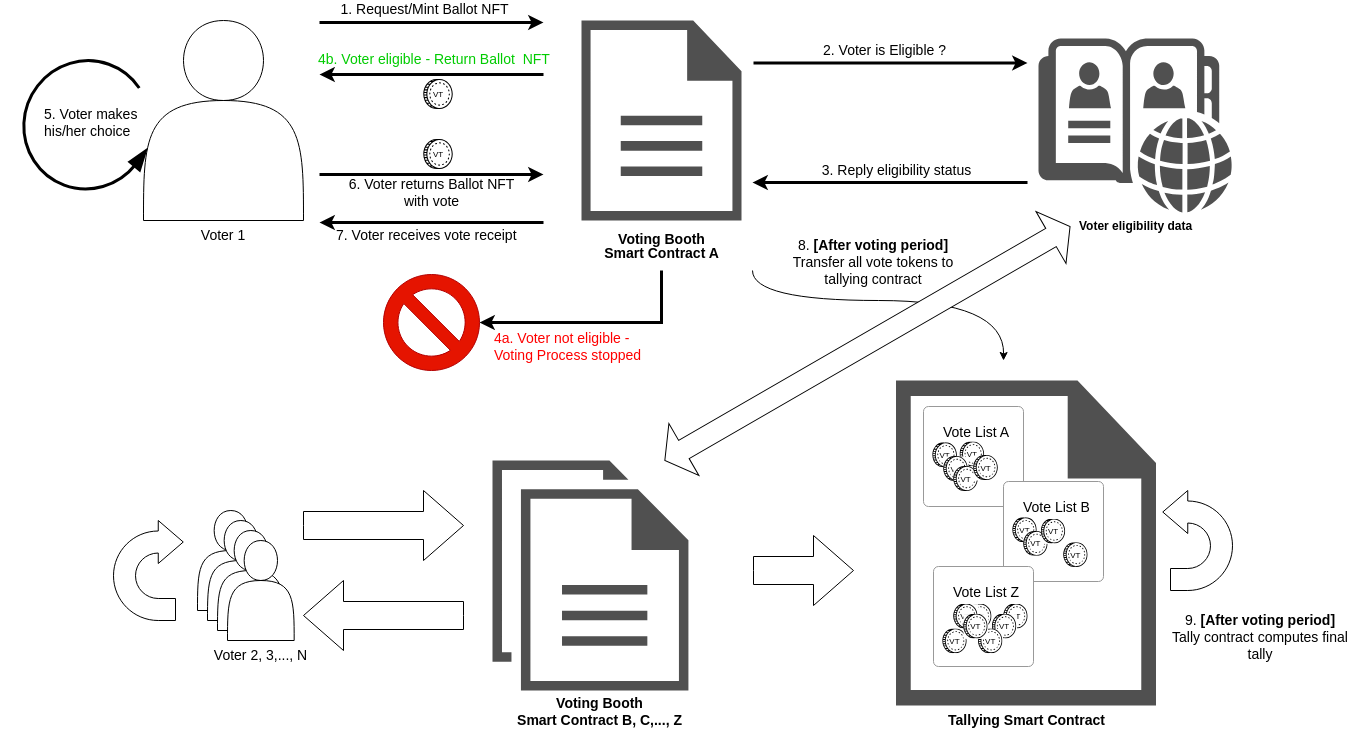
\includegraphics[width=0.7\textwidth]{../Images/03_account_based_solution.png}
    \caption{Account-based version of the e-voting system proposed.}
    \label{fig:account_based_architecture}
\end{figure}

In this scenario, each actor identified, namely the voters, the voting booth and tallying contracts, have their own accounts. Ballots are modeled as resources, as indicated in Section \ref{sec:resources_account_blockchains}, therefore they can only exist in one location, i.e., account, at a time, are not possible to copy, and only their owner can destroy them.
\par
The process starts with the voter interacting with a voting booth contract. The voter provides necessary information to determine his/her eligibility status in the present election, and if the query returns a positive outcome, the voting booth contract complies by minting a new Ballot NFT and transferring it to the voter. Next, the voter makes his/her selection by editing the token metadata accordingly and transfers the Ballot NFT back to the voting booth contract. All vote information is encrypted.
\par
The voting booth contract keeps all returned Ballot NFTs in its account storage until the end of the voting window. This allows for voters to be able to recast, or even revoke, their votes if desired. Once the election is over and the tally begins, voting booth contracts anonymise the Ballot NFTs, which locks the choices since these cannot be replaced or revoked anymore, and transfers all tokens to the tallying contract. This final contract removes the encryption layer, computes and publishes the results.

\end{document}